\chapter{Wybrany metoda symulacji ciała miękkiego}

\section{Kryteria wyboru modelu}

Wybór metody symulacji uzależniony jest od zakresu zjawisk fizycznych które mają
być jej przedmiotem. Zanim przedstawiona zostanie wybrana metoda wymienione będą
kryteria którymi kierowałem się przy jej wyborze.  Pragnę też zaznaczyć, że
wybór ten nastąpił w głównej mierze metodami prób i błędów.  Większość z
poznanych przeze mnie metod została zaimplementowana i w przypadku niemożności
uzyskania porządanych efektów wizualnych lub wydajnościowych wyszukiwana była
inna.

Pierwszym kryterium jakim kierowałem się przy wyborze metody było zawężenia
przedmiotu symulacji do ciał posiadających objętość. Wiele z metod symulacji
ciała miękkiego ukierunkowana jest na symulację ciał nie posiadających objętości
- takich jak włosy czy materiały. Metody te zaaplikowane do obiektów
posiadających objętość często nie dawały oczekiwanych rezultatów (miało to
		np. miejsce w przypadku omawianej później dyniamiki pozycyjnej w formie
		zaproponowanej przez jej autorów). Dodatkowo większość z posiadanych przez nie
własności trzeba było wyeliminować ze względu na charakter symulowanego zjawiska
- przykładem jest np. efekt marszczenia powierzchni.

Kolejnym kryterium, a właściwie uproszczeniem było założenie, że symulowany
obiekt będzie jednorodny pod względem wypełnienia, czy inaczej, materiału z
którego jest zbudowany. Pozwala to na uniknięcia modelowania, często
nietrywialnego, właściwości fizycznych modelu, co z pewnością wykroczyłoby poza
temat tej pracy. 

% złożone obiekty o skomplikowanej siatce
Innym istotnym wymaganiem jest umożliwienie symulowania obiektów
przygotowanych w programach do modelowania 3D. Obiekty takie często składają się
wielu tysięcy wierzchołków, które posiadają własne współrzędne teksturowania,
czy normalne. Implikacją tego założenia jest fakt, że poszukiwana metoda musi być
metodą Lagrange'a symulującą dynamikę wierzchołków trójwymiarowego modelu.
Dodatkowe informacje związane z modelem, takie jak połączenia między
wierzchołkami czy wierzchołki tworzące trójkąty mogą być wykorzystane w
symulacji.

% zakres degeneracji
Kolejnym wymaganiem jest przyjęcie, że symulowane ciało miękkie poddane
działaniu sił będzie odkształcane tylko w średnim zakresie. W
przypadku gdy siły zewnętrzne przestają działać na ciało, siły wewnętrzne
powinny sprowadzić obiekt do formy nieodkształconej. Takie założenie upraszcza
symulację gdyż wyklucza trwałą degenerację siatki obiektu.

% przeznaczona do symulacji czasu rzeczywistego stabilna do zastosowań
Najważniejszym wymaganiem jakie brane było pod uwagę przy wyborze metody jest możliwość
zastosowania jej do symulacji czasu rzeczywistego. Metody złożone obliczeniowo takie
jak przytaczane w rozdziale 2 Metody Continuum nie spełniają tego kryterium.
Również metody wymagające zaawansowanej obróbki modelu - taka jak np. System
Sprężyn wymagają zdefiniowania wewnętrznej struktury obiektu, co wiąże się z
generowaniem znacznej ilości cząstek poddanych symulacji. 

Z moich eksperymentów z wypełnianiem modelu sześcienną siatką i użyciem Systemu Sprężyn wynika, że
gęste wypełnienie średniej złożoności modelu punktami wewnętrznymi powoduje
zbytnie usztywnienie obiektu i znacząco spowalnia symulację. W przeciwieństwie,
gdy wnętrze modelu jest rzadko wypełnione cząstkami wewnętrznymi wyjściowa
siatka modelu podlega znacznej degeneracji. Znalezienie optymalnej gęstości
siatki oraz współczynników sprężystości sprężyn odbywało się drogą eksperymentów.

% skalowana do gpu
Tematem tej pracy jest również poznanie i zastosowanie technologii CUDA. Dlatego też
ostatnim kryterium jakie brane było pod uwagę przy wyborze metody symulacji jest
możliwość wykorzystania GPU do obliczeń.

% skad wzialem metode czyja to, kiedy skad
Jako źródło informacji o dostępnych metodach wykorzystywany był głównie
internet. Jak to zostało wcześniej napisane, nie są znane mi żadne książki
poruszające tematykę symulacji ciał miękkich w grafice komputerowej. Mimo
niedostępności poszukiwanego kompendium wiedzy dostępne są trzy bardzo dobre
artykuły stanowiące przekrój przez szereg opublikowanych metod: \cite{TR97-19},
	\cite{pbdo}, \cite{survey}. Cennym źródłem informacji są też materiały
	publikowane konferencyjne publikowane na stronie \textit{www.siggraph.org}.

% klasyfikacja tej metody - Lagrange geometryczno fizyczny
Zaimplementowana w tej pracy metoda bazuje na artykule \textit{Robust
	Real-Time Deformation of Incompressible Surface Meshes}\cite{diziol},
opublikowanym na konferencji SIGGRAPH w 2011r. Wybrana metoda jest wg
klasyfikacji z rozdziału 2 metodą Lagrange'a posiadająca zarówno elementy
fizyczne jak i niefizyczne. Elementami fizycznymi jest pojawianie się sił w
momencie gdy obiekt zmienia swoją objętość oraz siły grawitacji. Za część
niefizyczną, uznany jest tzw. \textit{Shape Matching}, czyli metoda geometryczna
oddziałująca na cząstki modelu w taki sposób aby zminimalizować ich odchylenie
ich położeń od stanu wejściowego oraz technika zachowania objętości. Obie
techniki będą dokładniej omawiane w rozdziałach \ref{sec:shape} i \ref{sec:vol}

% dlaczego powinna byc szybka nie potrzeba wypelniac obiektu puntkami - operuje bezposrednio na powierzchni siatki
Ważniejszą jednak zaletą wybranego modelu jest fakt, że w przeciwieństwie do
Systemu Sprężyn symulowane obiekty nie muszę mieć
zdefiniowanej struktury wewnętrznej. Pozwala to znacząco przyspieszyć symulację
unikając generowania i symulacji znacznej ilość cząstek, które odpowiadają tylko za
utrzymanie fizycznych właściwości obiektu. Metoda ta operuje bezpośrednio na
trójkątnej siatce, co pozawala wczytać obiekt bezpośrednio z formatu modeli
3D.

% dlaczego powinna byc stabilna - brak sil, dynamika z constraintami
Kolejną zaletą użytej techniki symulacji jest jej stabilność, która wynika z
nowatorskiego podejścia do rozwiązywania równań ruchu. Nie posiada ona
wielu typowych źródeł niestabilności typowych dla modelu Systemu Sprężyn.
Dokładne omówienie symulowania dynamiki wybranej metody nastąpi w rozdziale
\ref{sec:dyn}.

% dlaczego jest dobra na gpu
Ostatnią zaletą jest też możliwość efektywnej implementacji wybranej metody na
procesorach graficznych. Dobra lokalność przetwarzanych danych sprawia, że
możliwe jest pełne wykorzystanie procesora graficznego, co w połączeniu z
techniką redukcji złożoności algorytmu zaproponowaną przez autorów, czyni ją
idealną do zastosowania w symulacjach czasu rzeczywistego.

\section{Zachowanie kształtu}
\label{sec:shape}
Dopasowanie kształtu (ang. Shape Matching) jest geometryczną techniką
zaproponowaną po raz pierwszy w 2005 r. przez Muller'a \cite{shape}. Służy ona do
symulowania sił wewnętrznych ciała poddanemu deformacji. Metoda ta zamiast
generować siły działające na cząstki, tak jak to ma miejsce w przypadku
sprężyn w modelu Systemu Sprężyn, definiuje docelowe pozycje cząstek - $g_i$.
Pozycje te powstają w wyniku próby dopasowania konfiguracji 
pozycji cząstek ciała w stanie niezdeformowanym do aktualnej.

Wyliczone docelowe pozycje $g_i$ wykorzystywane są w symulacji do "przyciągania"
aktualnych pozycji cząstek. W przypadku gdy docelowe pozycje cząstek stają się
natychmiastowo aktualnymi uzyskamy efekt dynamiki ciała sztywnego.

\begin{figure}[ht]
\centering
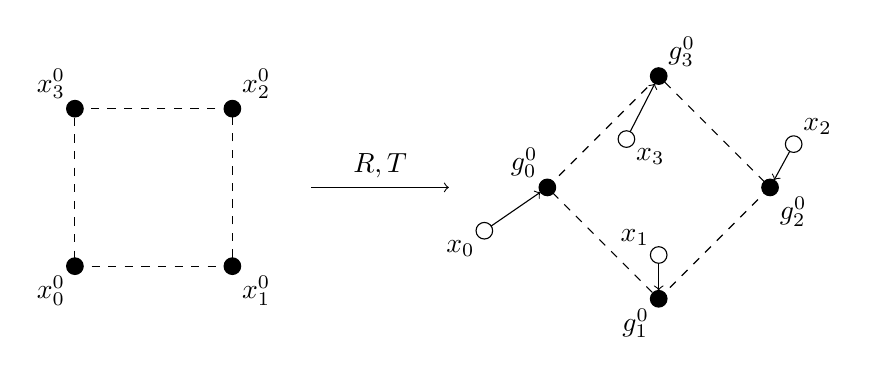
\begin{tikzpicture}

	\coordinate (A) at (0, 0, 0);
	\coordinate (B) at (2, 0, 0);
	\coordinate (C) at (2, 2, 0);
	\coordinate (D) at (0, 2, 0);

	\draw[-,dashed] (A) -- (B) -- (C) -- (D) -- (A);

	\filldraw[fill=black, draw=black] (A) circle (3pt);
	\filldraw[fill=black, draw=black] (B) circle (3pt);
	\filldraw[fill=black, draw=black] (C) circle (3pt);
	\filldraw[fill=black, draw=black] (D) circle (3pt);

	\node[above left] at (D) {$x^0_3$};
	\node[below right] at (B) {$x^0_1$};
	\node[above right] at (C) {$x^0_2$};
	\node[below left] at (A) {$x^0_0$};

	% arrow
	\coordinate (R1) at (3, 1, 0);
	\coordinate (R2) at (4.75, 1, 0);
    \draw[->] (R1) -- (R2) node[midway,above] {$R, T$};

	% transformed

	\coordinate (A1) at (6, 1, 0);
	\coordinate (B1) at (7.4142, 2.4142, 0);
	\coordinate (C1) at (8.8284, 1, 0);
	\coordinate (D1) at (7.4142, -0.4142, 0);

	\draw[-,dashed] (A1) -- (B1) -- (C1) -- (D1) -- (A1);

	\filldraw[fill=black, draw=black] (A1) circle (3pt);
	\filldraw[fill=black, draw=black] (B1) circle (3pt);
	\filldraw[fill=black, draw=black] (C1) circle (3pt);
	\filldraw[fill=black, draw=black] (D1) circle (3pt);

	\node[below left] at (D1) {$g^0_1$};
	\node[above right] at (B1) {$g^0_3$};
	\node[below right] at (C1) {$g^0_2$};
	\node[above left] at (A1) {$g^0_0$};

	\coordinate (X1) at (5.2, 0.45, 0);
	\coordinate (X2) at (7.0042, 1.6142, 0);
	\coordinate (X3) at (9.1284, 1.55, 0);
	\coordinate (X4) at (7.4142, 0.142, 0);

	\filldraw[fill=white, draw=black] (X1) circle (3pt);
	\filldraw[fill=white, draw=black] (X2) circle (3pt);
	\filldraw[fill=white, draw=black] (X3) circle (3pt);
	\filldraw[fill=white, draw=black] (X4) circle (3pt);

	\node[below left] at (X1) {$x_0$};
	\node[below right] at (X2) {$x_3$};
	\node[above right] at (X3) {$x_2$};
	\node[above left] at (X4) {$x_1$};

    \draw[shorten >=3pt,shorten <=3pt,->] (X1) -- (A1);
    \draw[shorten >=3pt,shorten <=3pt,->] (X2) -- (B1);
    \draw[shorten >=3pt,shorten <=3pt,->] (X3) -- (C1);
    \draw[shorten >=3pt,shorten <=3pt,->] (X4) -- (D1);

\end{tikzpicture}

\caption{Geometryczne dopasowanie kształtu do zdeformowanych punktów w Shape Matching.}
\label{shape-matching}
\end{figure}

Ideę shape matching przedstawia rysunek \ref{shape-matching}. Punkty w stanie
niezdeformowanym $x^0_i$ są dopasowywane do zdeformowanych pozycji $x_i$ za
pomocą macierzy rotacji i wektorów translacji. 
Formalnie koncepcję Shape Matchingu autorzy w \cite{shape} zdefiniowali jako problem minimalizacji
funkcji:
\begin{equation}
E^2 = \sum_{i} m_i ||R (x^0_i - t^0) - (x_i - t) ||^2,
\label{min}
\end{equation}
gdzie $t^0$ i $t_i$ są wektorami translacji, a $R$ jest macierzą
rotacji.

Przedstawiony w problem sprowadza się do minimalizacji błędu średniokwadratowego.
Wyrażenie z \ref{min} można przedstawić jako funkcję trzech zmiennych:
\begin{equation*}
\phi(R, t, t^0) = \sum_{i} m_i ||R (x^0_i - t^0) - (x_i - t) ||^2,
\end{equation*}

Okazuje się, że znalezienie wartości wektorów $t$ i $t^0$ w
wyrażeniu \ref{min} jest możliwe. Muller \cite{shape} podaje, że optymalnymi
wektorami translacji $t^0$ i $t$ są odpowiednio środek masy obiektu
niezdeformowanego (konfiguracja spoczynkowa) i środek masy
ciała w aktualnej konfiguracji. Pokazanie tego rozwiązania polega na
wyliczeniu gradientów funkcji $\phi$ po zmiennych $t$ i $t^0$ i przyrównaniu ich
do zera.

Zanim zostanie przedstawiony dowód że środki mas są optymalnymi wektorami
translacji, przypomniane zostaną wzory na pochodne cząstkowe wraz z ich
wektorowymi odpowiednikami. Zakładając że dane mamy funkcje $f: R^n \to R^m$,
$g: R^n \to R^m$ i $h = f^T g$, gdzie $h: R^n \to R^1$. Gradient
funkcji $h$ wyraża się wzorem:
\begin{equation*}
\partial h = f^T \partial g + g^T \partial f
\end{equation*}
gdzie $\partial f$ to macierz Jacobiego (pochodnych cząstkowych), a $f^T$ jest
oznaczeniem transpozycji funkcji.

W przypadku gdy funkcje $f = g$, gradient ma postać:
\begin{equation}
\partial h = 2 f^T \partial f,
\label{part}
\end{equation}

Wprowadzając nowe oznaczenia:
$$ v = R (x^0_i - t^0) - (x_i - t)$$
$$ \phi = \sum_i m_i v^T v$$ 
i uwzględniając własność \ref{part}, gradient funkcji $\phi$ po
zmiennych $t^0$ i $t$ zapiszemy:
\begin{eqnarray*}
\nabla_{t^0} \phi = 2 \sum_i m_i (R (x^0_i - t^0) + t - x_i)^T (-R)\\
\nabla_{t} \phi = 2 \sum_i m_i (R (x^0_i - t^0) + t - x_i)^T\\
\end{eqnarray*}

Transponując obie strony otrzymujemy:
\begin{eqnarray*}
\nabla_{t^0}^T \phi = -2 \sum_i m_i R^T (R (x^0_i - t^0) + t - x_i)\\
\nabla_{t}^T \phi = 2 \sum_i m_i (R (x^0_i - t^0) + t - x_i)\\
\end{eqnarray*}

W celu wyliczenia wartości $t$ i $t^0$ przyrównujemy gradient do zera:
\begin{eqnarray}
\label{d1}
\nabla \phi_{t^0} = 0 \Leftrightarrow \sum_i m_i R^T (R (x^0_i - t^0) + t - x_i) = 0\\
\label{d2}
\nabla \phi_{t} = 0 \Leftrightarrow \sum_i m_i R (x^0_i - t^0) + t - x_i = 0
\end{eqnarray}

Można łatwo zauważyć że równania \ref{d1} oraz \ref{d2} są od siebie liniowo
zależne. Przekształcając równanie \ref{d2} otrzymujemy:

\begin{eqnarray*}
\sum_i m_i (R (x^0_i - t^0) + t - x_i) = 0\\
\sum_i m_i R x^0_i - \sum_i m_i R t^0 + \sum_i m_i t - \sum_i m_i x_i = 0\\
R \sum_i m_i t^0 - \sum_i m_i t = R \sum_i m_i x^0_i - \sum_i m_i x_i\\
\end{eqnarray*}
Ostatecznie równanie spełniające warunek optymalizacji \ref{min} dla wektorów $t$
i $t^0$ możemy zapisać jako:
\begin{equation}
\label{tt0}
R t^0 - t = R \frac{\sum_i m_i x^0_i}{\sum_i m_i} - \frac{\sum_i m_i
	x_i}{\sum_i m_i}
\end{equation}

Z równania \ref{tt0} wynikają następujące wnioski. Nie istnieje unikalna para
wektorów
$t$ i $t^0$ spełniająca warunek minimalizacji wyrażenia \ref{min}. Rozwiązaniem
trywialnym \ref{tt0} jest $t = \frac{\sum_i m_i x_i}{\sum_i m_i}$
i $t^0 = \frac{\sum_i m_i x^0_i}{\sum_i m_i}$,
	co dowodzi tezy postawionej w \cite{shape}. Przyjęcie środków mas jako
	wektorów translacji sprawia, że wartości $t$ i $t^0$ minimalizujące
	\ref{min} są niezależne od wartości macierzy rotacji $R$.

Ostatnim elementem niezbędnym do wyliczenia docelowych pozycji $g_i$ jest
macierz obrotu $R$. W tym celu musimy wprowadzić następujące oznaczenia:
\begin{eqnarray*}
x_{cm}^0 = \frac{1}{M} \sum_i m_i x_i^0,\\
x_{cm} = \frac{1}{M} \sum_i m_i x_i,\\
M = \sum_i m_i,\\
\vec{q}_i = x_i^0 - x_{cm}^0,\\
\vec{p}_i = x_i - x_{cm}.
\end{eqnarray*}
Używając powyższych oznaczeń i uwzględniając fakt, że wybrane wektory translacji
są niezależne od R wyrażenie \ref{min} może być zapisane następująco:
\begin{equation*}
\phi(R) = \sum_i m_i || R\vec{q}_i - \vec{p}_i||^2
\end{equation*}

Wyznaczenie macierzy R odbywa się analogicznie jak w przypadku wektorów
translacji, z jedyną kompilacją, że gradient wyznaczony jest teraz po macierzy.
Muller \cite{shape} przy wyliczaniu macierzy $R$, uchyla założenie, że macierz ta
jest tylko macierzą rotacji, a przyjmuje, że jest to macierz transformacji
liniowej. W celu odróżnienia tych dwóch różnych problemów zdefiniujmy problem
ponownie jako:
\begin{eqnarray}
\phi(A) = \sum_i m_i || A \vec{q}_i - \vec{p}_i||^2
\end{eqnarray}

Rozwiązaniem minimalizującym funkcję $\phi$ jest macierz:\cite{shape}
\begin{equation}
A = (\sum_i m_i \vec{p}_i \vec{q}^T_i)(\sum_i m_i \vec{q}_i \vec{q}^T_i)^{-1}
= A_{pq} A_{qq}^{-1}
\end{equation}

Ostatnim krokiem niezbędnym do estymacji punktów docelowych $g_i$ jest
dekompozycja macierz $A$ i uzyskanie jest składowej rotacji. Jest to możliwe dzięki
użyciu metod takich jak Rozkład Biegunowy (Polar Decomposition) czy Rozkład
według wartości osobliwych (Singular Value Decomposition). Warto też nadmienić,
	że macierz $A_{qq}$ jest macierzą symetryczną i zawiera w sobie tylko
	informacje o skalowaniu, a cała informacja o rotacji jest obecna w
	macierzy $A_{pq}$

Zakładając że macierz $A_{pq}$ jest macierzą odwracalną, używając Rozkładu
Biegunowego możemy macierz zapisać jako:
\begin{equation}
A_{pq} = RS
\end{equation}
gdzie $R$ jest macierzą rotacji, a $S$ macierzą skalowania daną wzorami:
\begin{eqnarray*}
S = \sqrt[2]{A^T_{pq} A_{pq}}\\
R = A_{pq} S^{-1}
\end{eqnarray*}

%Formalnie pozycję $g_i$ wyraża się wzorem:
Ostatecznie pozycje docelowe $g_i$ można obliczyć jako:
\begin{equation}
g_i = R(x_i^0 - x^0_{cm}) + x_{cm}
\end{equation}

\subsection{Modyfikacje}
Shape Matching w swojej podstawowej formie dokonuje optymalizacji dopasowania
globalnie dla wszystkich punktów symulowanego ciała. Powoduje to jego zbytnie
usztywnienie i dopuszcza tylko wąski zakres deformacji.

Aby rozwiązać powyższe problemy Diziol w swoim artykule \cite{diziol} użył
lokalnego shape-matching. Autor unika globalnego dopasowania poprzez
predefiniowanie małych zbiorów sąsiadujących punktów w ramach których będzie
stosowany shape-matching.  W przypadku gdy cząstka należy do wielu regionów,
		  jako ostateczna docelowa pozycja $g_i$ używana jest średnia z
		  dopasowania z poszczególnych regionów.
\begin{equation}
g_i = \frac{1}{K_i} \sum_j^{K_i} R_j (x^0_i - x^0_{cm_j}) + x_{cm_j}
\end{equation}

\section{Zachowanie objętości}
\label{sec:vol}
Symulacja ciała miękkiego bez obostrzeń na zmiany objętości może
prowadzić do dużych jej zmian i niepożądanych wizualnie efektów. 
Aby temu zapobiec do modelu wprowadzona będzie siła wewnętrzna pojawiająca się w
przypadku gdy objętość ciała jest różna od objętości spoczynkowej oznaczonej
przez $V_0$.

Powierzchnię ciała o zamkniętej trójkątnej siatce określonej na jego powierzchni definiuje
się jako: \cite{diziol}
\begin{equation}
\label{obj}
\frac{1}{3} \sum_i^m A_i (a_i + b_i + c_i)^T n_i = 3V
\end{equation}
gdzie $m$ jest ilością trójkątów stanowiących siatkę, a punkty $a_i$, $b_i$,
	  $c_i$ wierzchołkami i-tego trójkąta, $A$ jego powierzchnią, a $n_i$
	  normalną trójkąta.

W pracy \cite{diziol} zdefiniowana jest funkcja ograniczenia nałożona na
objętość ciała postaci:
\begin{equation}
\label{cons}
C(X) = \frac{1}{3} \sum_i^m A_i (a_i + b_i + c_i)^T n_i - 3V_0 = 0
\end{equation}
gdzie $V_0$ jest objętością niezdeformowanego ciała, a $X$ jest zbiorem punktów
siatki. W przypadku gdy pewna konfiguracja punktów $\tilde{X} = [x_1, x_2,...,
	x_n] $ ciała generuje
objętość różną od $V_0$, wtedy należy znaleźć takie przesunięcie punktów $\Delta
\tilde{X}$, tak by spełniona była równość 
$$C(\tilde{X} + \Delta \tilde{X}) = 0$$

Funkcja ograniczenia \ref{cons} może zostać aproksymowana przez:
\begin{equation}
\label{e1}
C(X + \Delta X) \approx C(X) + \nabla_X C(X) \Delta X
\end{equation}

Zakładając, że przesunięcie $\Delta X$ może występować tylko wzdłuż gradientu $\nabla_X
C(X)$ otrzymujemy dodatkową równość:
\begin{equation}
\label{e2}
\Delta X = \lambda \nabla_X C(X)
\end{equation}

Rozwiązując układ równań \ref{e1} i \ref{e2} otrzymujemy ostateczną formułę
opisujące przemieszczenie $\Delta X$ rozwiązujące ograniczenie na objętość:
\begin{equation*}
\Delta X = - \frac{C(X)}{||\nabla_p C(X)||^2} \nabla_X C(X)
\end{equation*}

Indywidualne przemieszczenie $x_i$ mogą zostać wyliczone z formuły:
\begin{equation}
\Delta x_i = - \frac{C(X)}{\sum_j ||\nabla_{x_j} C(X)||^2} \nabla_{x_i} C(X)
\end{equation}

Aby ustalić wartość gradientu przekształcimy wyrażenie \ref{obj} w taki sposób,
	aby zamiast sumowania po trójkątach sumowała po punktach siatki:
\begin{equation}
\label{dd}
\frac{1}{3} \sum_i^m A_i (a_i + b_i + c_i)^T n_i = \frac{1}{3} \sum_i^n x_i^T
\tilde{n}_i
\end{equation}
gdzie $\tilde{n}_i = \sum_j A_j n_j$.

Diziol \cite{diziol} nie używa dokładnej formuły na gradient wyznaczony z
\ref{dd}. Zamiast tego proponuje następujące uproszczenie:
\begin{equation}
\nabla C(X) \approx \frac{1}{3} [\tilde{n}^T_1, \tilde{n}^T_2, ...,
	\tilde{n}^T_n]^T
\end{equation}
Według \cite{diziol} przybliżony gradient nie zmienia znacząco jego wartości, a
pozwala na łatwiejsze jego wyliczenia na GPU.

Ostateczną formułą na przesunięcie związane ze zmianą objętości możemy zapisać:
\begin{equation}
\delta x_i = \frac{\Delta V}{N} \tilde{n}_i
\end{equation}

%$$\iiint\limits_V \nabla \dot f(x) dx = \iint\limits_{\partial V} f(x)^T n(x) dx,$$

%$$\iiint\limits_V \nabla \dot x dx = \iint\limits_{\partial V} x^T n(x) dx = 3 V,$$

%$$ \iint\limits_{\partial V} x^T n(x) dx = \frac{1}{3} \sum_i^m A_i (a_i + b_i +
%		c_i)^T n_i,$$
%$$ \frac{1}{3} \sum_i^m A_i (a_i + b_i + c_i)^T n_i = \frac{1}{3}\sum_i^n x_i^T
%\tilde{n}_i,$$
\section{Dynamika bazująca na pozycji}
\label{sec:dyn}

Zastosowanie geometrycznych technik takich jak wymieniony w rozdziale
\ref{sec:shape} Shape-Matching czy metod zachowujących objętość w \ref{sec:vol}
jest problematyczne z tego względu, że siły działające na ciało nie wynikają
z nich bezpośrednio. Niemożliwe zatem jest jawne zdefiniowanie dynamiki układu
opisanego równaniem różniczkowym postaci $x\ddot{\vec{x}} = \vec{F}/m$.

Rozwiązaniem tego problemu może być emulowanie sił poprzez zaczepienie
'wirtualnych' sprężyn pomiędzy punktami docelowymi $g_i$ wynikającymi z ograniczeń
geometrycznych a aktualną pozycją $x_i$ cząstki. Otrzymane w ten sposób
siły działające na ciało mogą być użyte do rozwiązania równań ruchu.
Takie podejście nie jest jednak używane w literaturze przedmiotu. Zamiast tego
\cite{pbdyn} proponuje rozwiązanie postawionego problemu poprzez użycie
tzw. dynamiki bazującej na pozycjach (Position Based Dynamics).

Metody bazujące na pozycji są relatywnie młodą metodą wykorzystywaną w symulacji
ciał miękkich. Pierwsza propozycja takiego podejścia przedstawiona została w
2001 r.\cite{jak}, natomiast uogólniony, usystematyzowany koncept, został oficjalnie
opublikowany w 2006 r.\cite{pbdyn}. To właśnie autorom \cite{pbdyn} przypisuje
się odkrycie tej metody, która szybko stała się popularna w obszarze grafiki
komputerowej i jest dzisiaj implementowana w profesjonalnych silnikach fizycznych,
takich jak PhysX, Havoc Cloth, Maya nCloth czy Bullet \cite{Liu:2013:FSM}.

Termin bazujący na pozycji oznacza, że w odróżnieniu od modelu Systemu Sprężyn,
	   w którym to wyznaczenie kolejnych pozycji punktu w czasie $x_i(t +
			   \Delta t)$ jest zależne od sił wypadkowych działających na ten
	   punkt, do wyznaczania przyszłej pozycji w czasie $t + \Delta t$
	   wykorzystywana jest aktualna pozycja oraz jej tzw. projekcja. Jako
	   projekcję danego punktu $x_i$ rozumiana jest taka pozycja $g_i$, która
	   spełnia wszystkie obostrzenia (np. ograniczenia geometryczne)
	przewidziane w symulowanym modelu.

Bezpośrednie operowanie na pozycjach implikuje ważną własność metody. Odpowiednie
skonstruowanie funkcji obostrzeń i modyfikowanie wartości projekcji $g_i$, tak
aby były one spełnione, pozwala uniknąć typowych niestabilności związanych z
rozwiązaniem układu równań ruchu. Do takich niestabilności należy przede
wszystkim problem użycia zbyt dużego kroku symulacji $t$. Zbyt
duża wartość powoduje, że oscylacje sprężyn w modelu Systemu Sprężyn przejawiają
tendencje to tzw. overshootingu. Jest to zjawisko systematycznego powiększania rozciągnięcia
sprężyny w czasie oscylacji, powodujące błędny wzrost energii wewnętrznej układu i w
ostateczności jego widowiskową 'eksplozję'.

Do najważniejszych zalet Dyniamki bazującej na pozycji autorzy \cite{pbdyn}
zaliczają:
\begin{itemize}
	\item bezpośrednią kontrolę nad całkowaniem równań ruchu, pozwalającą
	rozwiązać problemy z niestabilnością modelu,
	\item punkty materialne mogą być bezpośrednio przesuwane, bez użycia sił,
	\item model ograniczeń bazujących na pozycji może być wykorzystany do
	symulowania szerokiego zakresu zdarzeń fizycznych,
	\item system rozwiązujący ograniczenia w modelu jest łatwy w implementacji.
\end{itemize}

\subsection{Definicja}
Dynamika pozycyjna zakłada, że każdy obiekt deformowalny jest przedstawiony jako zbiór $N$
punktów materialnych (zwanych dalej wierzchołkami) oraz $M$ ograniczeń
zdefiniowanych na tych wierzchołkach. Każdy i-ty wierzchołek symulowanego ciała posiada
następujące atrybuty:

\vspace{0.5cm}
\centering
\begin{tabular}{|r|l|}
\hline
$x_i$ & pozycja w $R^3$ \\
\hline
$v_i$ & prędkość \\
\hline
$m_i$ & masa\\
\hline
\end{tabular}
\vspace{0.5cm}

\raggedright
Ograniczenie, nazywane też wymiennie w tej pracy obostrzeniem,
posiada następujące atrybuty:
\vspace{0.5cm}

\centering
\begin{tabular}{|r|l|}
\hline
$n_j$ & liczność ograniczenia \\
\hline
$C_j$ & funkcja $R^{3n_j} -> R$\\
\hline
${i_1, ..., i_{n_j}}, i_k \in [1,..N]$ & zbiór indeksów\\
\hline
$k_j \in [0.. 1]$ & sztywność\\
\hline
typ & równość lub nierówność\\
\hline
\end{tabular}
\vspace{0.5cm}

\raggedright
Liczność ograniczenia $n_j$ informuje ile wierzchołków danego symulowanego ciała 
podlega temu ograniczeniu. Funkcja $C_j : R^{3n_j} -> R$ będzie używana do
określenia czy dane ograniczenie jest spełnione oraz do wyznaczania docelowych
przesunięć wierzchołków $\Delta X$ spełniających warunek $C_j(X + \Delta X) = 0$. 
Lista indeksów służy przypisaniu konkretnych wierzchołków do danego
ograniczenia.

Parametr $k_j$ informuje o tym jak szybko dane ograniczenie ma
powodować zmianę konfiguracji punktów projekcji $g_i$. Po wyznaczeniu
optymalnej pozycji punktów $X + \Delta X$ pozycje $g_i$ są przesuwane w kierunku
docelowych punktów, przeskalowanym o parametr $k_j$. Możemy to zapisać jako:
$$g'_i = g_i + k_j ((x_i + \Delta x_i) - g_i)$$
W efekcie parametr $k_j$ służy do symulowania fizycznych właściwości
będących efektem działania ograniczenia. Dla $k_j \to 1$ uzyskamy zatem
zachowanie przypominające ciało sztywne, natomiast przy $k_j \to 0$ uzyskamy
efekt całkowitego zaniku sił wewnętrznych podczas deformacji ciała.

Ostatnim atrybutem obostrzenia jest jego typ - przyjmujący wartości równość lub
nierówność.  Jeżeli ograniczenie jest typu równości to spełnione jest wówczas
wtedy gdy $C_j(x_{i_1},..., x_{i_{n_j}}) = 0$, natomiast dla typu nierówność to
wtedy gdy $C_j(x_{i_1},..., x_{i_{n_j}}) > 0$.
Przykładem obostrzeń typu równość jest zachowanie odległości między dwoma
wierzchołkami ciała miękkiego:
\begin{equation}
C(x_i, x_j) = || x_i - x_j || - l_{ij} = 0
\end{equation}
gdzie $l_{ij}$ jest odległością między wierzchołkami i, j w niezdeformowanej
konfiguracji wierzchołków.

Przykładem ograniczenia typu nierówność może być kolizja z płaszczyzną, która
w swojej najprostszej postaci może mieć postać:
\begin{equation}
C(x_i) = (x - \vec{p}) \circ \vec{n} > 0
\end{equation}
gdzie $\vec{p}$ jest punktem leżącym na płaszczyźnie, a $\vec{n}$ jest normalną
płaszczyzny.

Dynamika pozycyjna pomimo faktu, że stworzona została z myślą o ograniczeniach
geometrycznych pozwala także wprowadzić do modelu wpływ działania tradycyjnych sił takich jak grawitacja
czy siła wiatru. Możliwe jest to dzięki przyjęciu, że początkowe wartości
projekcji $g_i$ są wyznaczone dzięki tradycyjnemu rozwiązaniu równań ruchu z
modelu Systemu Sprężyn postaci $x \ddot{\vec{x}} = \vec{F} / m$.

Zasadniczą ideą Dynamiki Pozycyjnej jest iteracyjne rozwiązywanie
równań ograniczeń zdefiniowanych dla modelu.
Dzieje się to poprzez systematyczne sprawdzanie zdefiniowanych ograniczeń i w
przypadku gdy nie jest ono spełnione dokonywane jest rzutowanie punktów $g_i$ na
nowe pozycje (przy uwzględnieniu parametru $k$). Aby zobrazować idę
Position Based Dynamics przedstawiony zostanie oryginalny algorytm zaproponowany
przez autorów w \cite{pbdyn}.

\paragraph{Algorytm}

Mając dany zbiór wierzchołków modelu, zbiór ograniczeń i krok symulacji $\{X_N,
	C_M, \Delta t \}$, algorytm przebiega następująco:
\begin{enumerate}
\item \textbf{for} $i = 1:N$
\item \hspace{1cm} $x_i = x_i^0, v_i = v_i^0, w_i = 1/m_i$
\item \textbf{end for}
\item \textbf{loop}
\item \hspace{1cm} \textbf{for} $i = 1:N$ \textbf{do} $v_i \leftarrow v_i + \Delta t w_i f_{ext}(x_i)$
\item \hspace{1cm} \textbf{for} $i = 1:N$ \textbf{do} $g_i \leftarrow x_i + \Delta t v_i$
\item \hspace{1cm} \textbf{for} $j = 1:liczbaIteracji$
\item \hspace{2cm} $rozwiazOgrnaiczenia(C_1,..., C_{M}, g_1, ..., g_N)$
\item \hspace{1cm} \textbf{end for}
\item \hspace{1cm} \textbf{for} $i = 1:N$
\item \hspace{2cm} $v_i = (g_i - x_i) / \Delta t$
\item \hspace{2cm} $x_i = g_i$
\item \hspace{1cm}\textbf{end for}
\item \textbf{end loop}

\end{enumerate}

W zaproponowanej przez Mullera algorytmie, najważniejszą część stanowią
fragmenty (6), (8), 11-12. W linii (6) następuje całkowanie równania ruchu za 
pomocą metody Eulera. Ustala się w ten sposób pierwszą projekcję pozycji $g_i$. Następnie
wszystkie projekcje są rzutowane w taki sposób rozwiązywały one
ograniczenia $C_M$. Należy tutaj zaznaczyć, że w algorytmie nie zakłada się, że
ograniczenia $C(g)$ będą rozwiązane dokładnie. Spowodowałoby to 
usztywnienie systemu i niepożądane wizualnie efekty. Dlatego też każde
ograniczenie zostanie rozwiązane z pewnym błędem zależnym od parametru $k$ oraz
ilości iteracji rozwiązania ograniczeń.
Ostatnim krokiem symulacji jest ponowne obliczenie
prędkości oraz przypisane zrzutowanej projekcji do pozycji wierzchołka.

Przedstawiona symulacja jest bezwarunkowo stabilna \cite{pbdyn} ponieważ nowe pozycje nie są
ekstrapolacją wynikająca z kroku całkowania (6), tyko pewnym rzutowaniem na
stabilne konfiguracje systemu wynikające z równań ograniczeń (8). Jedynym
źródłem niestabilności jest sam proces rozwiązywania ograniczeń \cite{pbdyn}
Jednakże niestabilność nie zależy od przyjętego kroku całkowania systemu $\Delta
t$, tylko od samej funkcji danego ograniczenia\cite{pbdyn}.

\subsection{Rozwiązywanie układu ograniczeń}
Problem rozwiązania ograniczeń $C_1, .., C_M$ dla projekcji układu $g_1, ..., g_N$
jest w istocie problemem rozwiązania układu równań. Do rozwiązania takiego
układu autorzy sugerują posłużyć się metdoą Jacobiego bądź metodą Gaussa-Seidela. 

Wyżej wymienione metody mogą mieć zastosowanie tylko w przypadku
liniowych układów równań. Niestety w modelu funkcje ograniczeń mają też postać nierówności, a
najczęściej spotykane funkcje ograniczeń mają charakter nieliniowy. Powoduje to,
że niemożliwe jest użycie klasycznych wersji w/w metod. Muller proponuje
zmodyfikowana metodę Gaussa-Seidela, w której każde równanie (lub nierówność) będzie rozwiązane
oddzielnie metodą Newtona, a następnie zmodyfikowana projekcja będą używana do
rozwiązania kolejnych równań ograniczeń.

\subsection{Przykłady ograniczeń}
Ograniczenia mają za cel zdefiniowanie przestrzeni rozwiązań możliwych w której
znaleźć mogą się projekcje $g$.  Jeżeli dane ograniczenie modeluje siły
wewnętrzne między punktami należącymi do obiektu to przesunięcie $\Delta g$,
	które będzie efektem jego rozwiązania dla danej konfiguracji $g$ musi
	posiadać pewne pożądane z punktu widzenia symulacji własności: zachowanie
	pędu oraz momentu pędu.

Pęd jest zachowany jeśli przesunięcie $\Delta g$ posiada własność:
$$ \sum_i m_i \Delta g_i = 0$$
Natomiast moment pędu jest zachowany gdy:
$$ \sum_i r_i \times m_i \Delta g_i = 0$$
gdzie $r_i$ jest odległością $g_i$ do osi
obrotu.

Nie spełnienie w/w równości skutkuje powstawaniem dodatkowych sił, które
oddziałują na punkty obiektu, tak jak siły zewnętrzne. Jeżeli dane ograniczenie
dotyczy zewnętrznych właściwości (np. odległości od punktu kolizji),
własności te nie muszą być zachowane\cite{pbdyn}.

Muller proponuje następujący wzór na obliczanie przemieszczenie $\Delta g$ dla
ograniczeń zachowujący jednocześnie pęd jak i moment pędu.
Jeżeli $g = [ g_1^T, g_2^T, ..., g_n^T]^T$, gdzie $n$ jest licznością
ograniczenia $C$:
\begin{equation} \label{con_eq}
\Delta g = - \frac{C(g)}{|| \nabla_g C(g) ||^2}\nabla_g C(g),
\end{equation}
a $\nabla_g C(g)$ jest gradientem dla ograniczenia $C$ w $g$.

Przemieszczenie dla poszczególnego wierzchołka wyraża się wzorem:
$$\Delta g_i = -s w_i\nabla_{g_i}C(g_1, ..., g_n)$$ 
$$ s = \frac{C(g_1, ..., g_n)}{\sum_j w_j|| \nabla_{g_j}C(g_1, ..., g_n)
	||^2}$$

gdzie $w_i = 1 / m_i$

Przedstawiona powyżej projekcja jest przeprowadzana w kroku (8) głównego
algorytmu dla każdego ograniczenia $C_i$ o typie równości.
W przypadku gdy typ ograniczenia jest nierównością przemieszczenie $g$
o wyliczony wektor $\Delta g$ następuje tylko wtedy, gdy $C(g_1, ...,
		g_n) < 0$.

\paragraph{Dystans między punktami}
Ograniczenie w dystansie między punktami pozwala symulować efekt efekt działania
sił wewnętrznych. W swojej podstawowej wersji funkcja ograniczenia dana jest wzorem:
$$ C(g_1, g_2) = || g_1 - g_2 || - d,$$ 
gdzie $d$ jest wartością
spoczynkową, czyli odległością między punktami $g_1$ i $g_2$ w stabilnej
konfiguracji.

Funkcja ograniczenia spełnia warunek dla wzoru \ref{con_eq}, czyli jest
niezależna od translacji i obrotu punktów (zachowuje pęd i moment pędu).
Dlatego też wzór na korekta projkcji dla
ograniczenia dystansu jest równa:

$$\Delta g_1 = - \frac{w_1}{w_1 + w_2} (|| g_1 - g_2 || - d)\frac{g_1 -
	g_2}{|| g_1 - g_2 ||}$$

$$\Delta g_2 = + \frac{w_2}{w_1 + w_2} (|| g_1 - g_2 || - d)\frac{g_1 -
	g_2}{|| g_1 - g_2 ||}$$

Aby otrzymać ostateczną korektę projekcji $g_1$ i $g_2$ w,
	trzeba otrzymane wartości $\Delta g_1$ oraz $\Delta g_2$ pomnożyć przez
	sztywność ograniczenia $k$, gdzie $k \in (0, 1)$. 
	$$ g_i = g_i + k * \Delta g_i$$
Powyższe równanie ma jedną niepożądaną własność, ostatecznie przesunięcie
$\Delta g_i$ jest zależne od ilości iteracji rozwiązania równań ograniczeń.
Efekt po $I$ iteracjach na ostateczne przesunięcie $\Delta p$ będzie
nieliniowy i równy $\Delta g_0 k^I$. Aby pozbyć się zależności od liczby
iteracji, parametr $k$ musi być funkcją $I$, czyli: $$ k' = 1 - (1 -
		k)^{1/I}$$

